\documentclass{beamer}

\usepackage{epsfig,graphicx,parskip,setspace,tabularx,xspace,url,holtexbasic,alltt,proof,tikz}
\usetikzlibrary{arrows}
\usetikzlibrary{positioning}
\usetheme{CambridgeUS}

\title[Verified register allocation]{Developing a formally verified algorithm for register allocation}
\subtitle{A Part III project}
\author{David Barker}
\date{9\textsuperscript{th} June 2014}
\subject{Computer Science}


\begin{document}

\frame{\titlepage}

\section{Introduction}

\begin{frame}
\frametitle{The problem of register allocation}

\begin{itemize}
	\item Intermediate code assumes infinite registers
	\item Real machines have finite registers
	\item Using memory costs many cycles
\end{itemize}
\end{frame}

\subsection{Register allocation by graph colouring}
\begin{frame}
\frametitle{Computing live ranges}
\end{frame}

\begin{frame}
\frametitle{Building a clash graph}
\end{frame}

\begin{frame}
\frametitle{Colouring the clash graph}
\end{frame}

\begin{frame}
\frametitle{Applying the colouring}
\end{frame}

\begin{frame}
\frametitle{The full algorithm}

\begin{columns}[c]
\column{.5\textwidth}
 \begin{center}
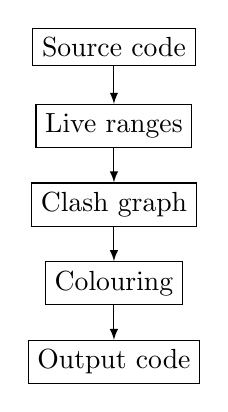
\begin{tikzpicture}[node distance = 1cm, auto]
    % Place nodes
    \node [draw] (source) {Source code};
    \node [draw, below of=source] (live) {Live ranges};
    \node [draw, below of=live] (graph) {Clash graph};
    \node [draw, below of=graph] (colouring) {Colouring};
    \node [draw, below of=colouring] (code) {Output code};
    % Draw edges
    \draw [-latex] (source) -- (live);
    \draw [-latex] (live) -- (graph);
    \draw [-latex] (graph) -- (colouring);
    \draw [-latex] (colouring) -- (code);
\end{tikzpicture}
\end{center}
\column{.5\textwidth}
 A correct algorithm will generate output code with exactly the same behaviour
\end{columns}
\end{frame}

\subsection{Guaranteeing correctness}
\begin{frame}[containsverbatim]
\frametitle{How we ensure this behaviour}
A correct algorithm produces a colouring which causes no conflicts between simultaneously live registers:

\begin{alltt}\small
	\HOLConst{colouring_ok_alt} \HOLFreeVar{c} \HOLFreeVar{code} \HOLFreeVar{live} \HOLTokenEquiv{}
\HOLConst{colouring_respects_conflicting_sets} \HOLFreeVar{c}
  (\HOLConst{conflicting_sets} \HOLFreeVar{code} \HOLFreeVar{live})
\end{alltt}

This was proved sufficient: a colouring satisfying this will always yield code with unchanged behaviour
\end{frame}

\section{Modelling the problem}
\begin{frame}[containsverbatim]
\frametitle{Code representation}
A block of code is represented by a list of three-address instructions:

\begin{alltt}\small
	\HOLTyOp{inst} = \HOLConst{Inst} \HOLKeyword{of} \HOLTyOp{num} \HOLTokenImp{} \HOLTyOp{num} \HOLTokenImp{} \HOLTyOp{num}
\end{alltt}

This is evaluated on a store $s$ as follows:

\begin{alltt}\small
	\HOLConst{eval} \HOLFreeVar{f} \HOLFreeVar{s} [] = \HOLFreeVar{s}
\HOLConst{eval} \HOLFreeVar{f} \HOLFreeVar{s} (\HOLConst{Inst} \HOLFreeVar{w} \HOLFreeVar{r\sb{\mathrm{1}}} \HOLFreeVar{r\sb{\mathrm{2}}}::\HOLFreeVar{code}) =
\HOLConst{eval} \HOLFreeVar{f} ((\HOLFreeVar{w} =+ \HOLFreeVar{f} (\HOLFreeVar{s} \HOLFreeVar{r\sb{\mathrm{1}}}) (\HOLFreeVar{s} \HOLFreeVar{r\sb{\mathrm{2}}})) \HOLFreeVar{s}) \HOLFreeVar{code}
\end{alltt}
\end{frame}

\begin{frame}[containsverbatim]
Colourings are functions of type $num \rightarrow num$

Colourings can be applied simply by substituting registers:

\begin{alltt}\small
	\HOLConst{apply} \HOLFreeVar{c} [] = []
\HOLConst{apply} \HOLFreeVar{c} (\HOLConst{Inst} \HOLFreeVar{w} \HOLFreeVar{r\sb{\mathrm{1}}} \HOLFreeVar{r\sb{\mathrm{2}}}::\HOLFreeVar{code}) =
\HOLConst{Inst} (\HOLFreeVar{c} \HOLFreeVar{w}) (\HOLFreeVar{c} \HOLFreeVar{r\sb{\mathrm{1}}}) (\HOLFreeVar{c} \HOLFreeVar{r\sb{\mathrm{2}}})::\HOLConst{apply} \HOLFreeVar{c} \HOLFreeVar{code}
\end{alltt}
\end{frame}

\begin{frame}[containsverbatim]
\frametitle{Set representation}
To simplify definitions and proofs, sets are represented as duplicate-free lists and all functions manipulating them are proven to preserve duplicate-freeness

Simple set functions:

\begin{alltt}\small
	\HOLConst{insert} \HOLFreeVar{x} \HOLFreeVar{xs} = \HOLKeyword{if} \HOLConst{MEM} \HOLFreeVar{x} \HOLFreeVar{xs} \HOLKeyword{then} \HOLFreeVar{xs} \HOLKeyword{else} \HOLFreeVar{x}::\HOLFreeVar{xs}
\end{alltt}

\begin{alltt}\small
	\HOLConst{delete} \HOLFreeVar{x} \HOLFreeVar{xs} = \HOLConst{FILTER} (\HOLTokenLambda{}\HOLBoundVar{y}. \HOLFreeVar{x} \HOLTokenNotEqual{} \HOLBoundVar{y}) \HOLFreeVar{xs}
\end{alltt}

\begin{alltt}\small
	\HOLConst{list_union} [] \HOLFreeVar{ys} = \HOLFreeVar{ys}
\HOLConst{list_union} (\HOLFreeVar{x}::\HOLFreeVar{xs}) \HOLFreeVar{ys} = \HOLConst{insert} \HOLFreeVar{x} (\HOLConst{list_union} \HOLFreeVar{xs} \HOLFreeVar{ys})
\end{alltt}

\begin{alltt}\small
	\HOLConst{list_union_flatten} [] = []
\HOLConst{list_union_flatten} (\HOLFreeVar{l}::\HOLFreeVar{ls}) =
\HOLConst{list_union} \HOLFreeVar{l} (\HOLConst{list_union_flatten} \HOLFreeVar{ls})
\end{alltt}
\end{frame}

\section{The algorithm}
\subsection{Live variable analysis}

\begin{frame}[containsverbatim]
\frametitle{Live variable analysis}
The set of live variables before a block of code is given by the following equation:

\begin{center}
$live(n) = \left(live(n+1) \setminus write(n)\right) \cup read(n)$
\end{center}

This was implemented as follows:

\begin{alltt}\small
	\HOLConst{get_live} [] \HOLFreeVar{live} = \HOLFreeVar{live}
\HOLConst{get_live} (\HOLConst{Inst} \HOLFreeVar{w} \HOLFreeVar{r\sb{\mathrm{1}}} \HOLFreeVar{r\sb{\mathrm{2}}}::\HOLFreeVar{code}) \HOLFreeVar{live} =
\HOLConst{insert} \HOLFreeVar{r\sb{\mathrm{1}}} (\HOLConst{insert} \HOLFreeVar{r\sb{\mathrm{2}}} (\HOLConst{delete} \HOLFreeVar{w} (\HOLConst{get_live} \HOLFreeVar{code} \HOLFreeVar{live})))
\end{alltt}
\end{frame}

\begin{frame}[containsverbatim]
\frametitle{Correctness}
This was implicitly proved correct as its usage led to an algorithm proven to generate behaviour-preserving colourings

More directly, it was proved that only registers returned by \texttt{get\_live} affect program behaviour:

\begin{alltt}\small
	(\HOLConst{MAP} \HOLFreeVar{s} (\HOLConst{get_live} \HOLFreeVar{code} \HOLFreeVar{live}) = \HOLConst{MAP} \HOLFreeVar{t} (\HOLConst{get_live} \HOLFreeVar{code} \HOLFreeVar{live})) \HOLTokenImp{}
(\HOLConst{MAP} (\HOLConst{eval} \HOLFreeVar{f} \HOLFreeVar{s} \HOLFreeVar{code}) \HOLFreeVar{live} = \HOLConst{MAP} (\HOLConst{eval} \HOLFreeVar{f} \HOLFreeVar{t} \HOLFreeVar{code}) \HOLFreeVar{live})
\end{alltt}
\end{frame}


\end{document}